\documentclass[12pt, a4paper]{article}

% --- Packages ---
\usepackage[utf8]{inputenc}
\usepackage[T1]{fontenc}
\usepackage{geometry}
\usepackage{titlesec}
\usepackage{enumitem}
\usepackage{booktabs}
\usepackage{hyperref}
\usepackage{graphicx}
\usepackage{amsmath}
\usepackage{xcolor}
\usepackage{longtable}
\usepackage{array}
\usepackage{tabularx}
\usepackage{tikz}
\usepackage{pgfgantt}
\usetikzlibrary{shapes.geometric, arrows.meta, positioning, fit, backgrounds}

\geometry{margin=1in}

\hypersetup{
    colorlinks=true,
    linkcolor=blue,
    urlcolor=blue,
    citecolor=blue
}

% --- Title ---
\title{
    \textbf{Project Proposal:} \\[0.5em]
    Predicting the Effectiveness of Crowd-Sourced Fact-Checking Using Fine-Tuned LLMs --- A Study on Twitter/X Community Notes
}
\author{Md Shahidul Salim \and Rafa Pashkov \and Mridul Madan}
\date{}

\begin{document}

\maketitle

% ============================================================
\section{Project Overview}
% ============================================================

\textbf{Core Idea:} Twitter/X's \textbf{Community Notes} (formerly Birdwatch) allows users to collaboratively write fact-checking notes on potentially misleading tweets. Notes rated ``Helpful'' by a diverse set of raters are displayed publicly. This project will \textbf{fine-tune LLMs to predict whether a Community Note will be rated ``Helpful,''} analyze what linguistic features make notes effective, and compare fine-tuning approaches with prompting baselines.

\medskip
\noindent\textbf{Why This Is Unique \& Strong:}
\begin{itemize}[nosep]
    \item Sits squarely in \textbf{social computing} (crowdsourcing, collective intelligence, platform governance, content moderation)
    \item Publicly available, regularly updated, large-scale dataset directly from Twitter/X
    \item Understudied with modern LLMs --- most existing work focuses on the ranking algorithm, not content-based prediction
    \item Directly leverages our LLM fine-tuning and inference expertise
    \item High real-world impact (improving misinformation countermeasures)
\end{itemize}

% ============================================================
\section{Introduction}
% ============================================================

Misinformation on social media is one of the most pressing socio-technical challenges of the modern era. Traditional fact-checking by professional organizations is slow, expensive, and cannot scale to the volume of content posted daily. Twitter/X's \textbf{Community Notes} program offers a novel crowd-sourced alternative: everyday users write contextual notes for potentially misleading tweets, and these notes are evaluated by other contributors. A note is shown publicly only if it is rated ``Helpful'' by raters who span diverse viewpoints --- a mechanism designed to surface notes that bridge ideological divides rather than reinforce partisan positions~\cite{allen2022}.

Despite the growing importance of Community Notes as a content moderation mechanism, relatively little computational work has focused on \textbf{predicting note effectiveness from textual content alone}. Most existing research examines the platform's bridging-based ranking algorithm~\cite{allen2022} or studies aggregate effects on engagement~\cite{chuai2024}. Understanding \emph{what makes a fact-checking note linguistically effective} is crucial for (a)~training future contributors, (b)~providing real-time feedback during note drafting, and (c)~designing better crowd-sourced moderation systems.

We propose to \textbf{fine-tune open-source large language models} (Qwen3-4B-Instruct, Gemma-3-4B-IT) to predict whether a Community Note will achieve ``Currently Rated Helpful'' status. Fine-tuning will be performed using \textbf{Unsloth AI}~\cite{unsloth} for efficient LoRA adaptation, and inference will be powered by \textbf{vLLM}~\cite{vllm} for high-throughput serving. We will compare fine-tuned models against traditional ML baselines (TF-IDF + Logistic Regression, BERT-base) and prompting-based approaches (zero-shot, few-shot, chain-of-thought). Additionally, we will conduct a qualitative analysis of the linguistic strategies that distinguish effective from ineffective notes, examining how factors such as source citation, neutral tone, and specificity influence note success.

\textbf{Beneficiaries} include platform designers, content moderation researchers, policy makers studying misinformation countermeasures, and Community Notes contributors themselves.

% ============================================================
\section{Project Workflow}
% ============================================================

Figure~\ref{fig:workflow} illustrates the end-to-end workflow of our project, from data collection through final analysis.

\begin{figure}[h!]
\centering
\resizebox{\textwidth}{!}{%
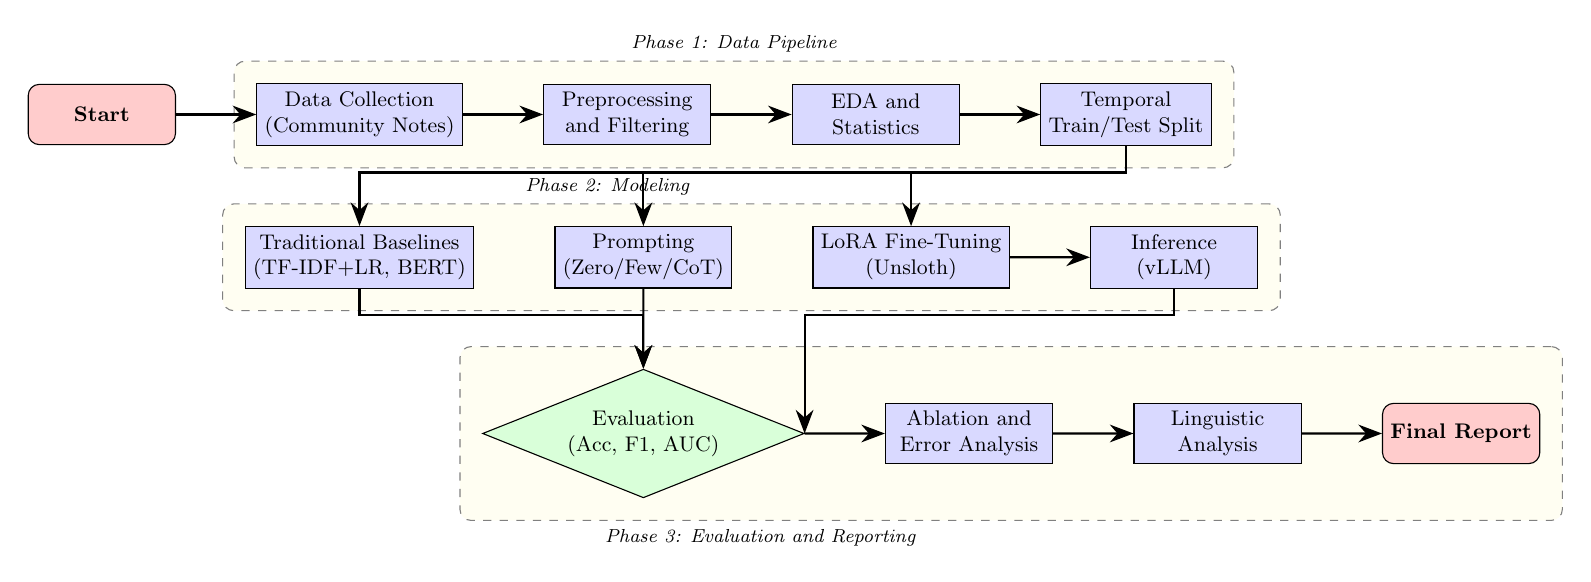
\begin{tikzpicture}[
    scale=0.85, transform shape,
    node distance=0.6cm and 1.2cm,
    startstop/.style={rectangle, rounded corners, minimum width=2.2cm, minimum height=0.9cm, align=center, draw=black, fill=red!20, font=\small\bfseries},
    process/.style={rectangle, minimum width=2.5cm, minimum height=0.9cm, align=center, draw=black, fill=blue!15, font=\small},
    decision/.style={diamond, minimum width=2cm, minimum height=0.9cm, align=center, draw=black, fill=green!15, font=\small, aspect=2.5},
    arrow/.style={-{Stealth[length=3mm]}, thick},
    groupbox/.style={draw=gray, dashed, rounded corners, inner sep=8pt, fill=yellow!5}
]
% Row 1: Data Pipeline
\node (start) [startstop] {Start};
\node (collect) [process, right=of start] {Data Collection\\(Community Notes)};
\node (preprocess) [process, right=of collect] {Preprocessing\\and Filtering};
\node (eda) [process, right=of preprocess] {EDA and\\Statistics};
\node (split) [process, right=of eda] {Temporal\\Train/Test Split};

% Row 2: Model approaches (below)
\node (baseline) [process, below=1.2cm of collect] {Traditional Baselines\\(TF-IDF+LR, BERT)};
\node (prompting) [process, right=of baseline] {Prompting\\(Zero/Few/CoT)};
\node (finetune) [process, right=of prompting] {LoRA Fine-Tuning\\(Unsloth)};
\node (inference) [process, right=of finetune] {Inference\\(vLLM)};

% Row 3: Evaluation
\node (eval) [decision, below=1.2cm of prompting] {Evaluation\\(Acc, F1, AUC)};
\node (ablation) [process, right=of eval] {Ablation and\\Error Analysis};
\node (linguistic) [process, right=of ablation] {Linguistic\\Analysis};
\node (report) [startstop, right=of linguistic] {Final Report};

% Arrows: Row 1
\draw [arrow] (start) -- (collect);
\draw [arrow] (collect) -- (preprocess);
\draw [arrow] (preprocess) -- (eda);
\draw [arrow] (eda) -- (split);

% Arrows: Row 1 to Row 2
\draw [arrow] (split.south) -- ++(0,-0.4) -| (baseline.north);
\draw [arrow] (split.south) -- ++(0,-0.4) -| (prompting.north);
\draw [arrow] (split.south) -- ++(0,-0.4) -| (finetune.north);

% Arrows: Row 2
\draw [arrow] (finetune) -- (inference);

% Arrows: Row 2 to Row 3
\draw [arrow] (baseline.south) -- ++(0,-0.4) -| (eval.north);
\draw [arrow] (prompting.south) -- (eval.north);
\draw [arrow] (inference.south) -- ++(0,-0.4) -| (eval.east);

% Arrows: Row 3
\draw [arrow] (eval) -- (ablation);
\draw [arrow] (ablation) -- (linguistic);
\draw [arrow] (linguistic) -- (report);

% Group boxes
\begin{scope}[on background layer]
    \node[groupbox, fit=(collect)(preprocess)(eda)(split), label={[font=\footnotesize\itshape]above:Phase 1: Data Pipeline}] {};
    \node[groupbox, fit=(baseline)(prompting)(finetune)(inference), label={[font=\footnotesize\itshape]above left:Phase 2: Modeling}] {};
    \node[groupbox, fit=(eval)(ablation)(linguistic)(report), label={[font=\footnotesize\itshape]below left:Phase 3: Evaluation and Reporting}] {};
\end{scope}
\end{tikzpicture}%
}
\caption{End-to-end project workflow.}
\label{fig:workflow}
\end{figure}

% ============================================================
\section{Dataset}
% ============================================================

We use the \textbf{publicly available Community Notes dataset} released by Twitter/X (\url{https://communitynotes.twitter.com/guide/en/under-the-hood/download-data}), which is updated daily and consists of three TSV files:

\begin{table}[h!]
\centering
\begin{tabularx}{\textwidth}{l X c}
\toprule
\textbf{File} & \textbf{Description} & \textbf{Approx.\ Size} \\
\midrule
\texttt{notes-00000.tsv} & All notes with text, classification, metadata & $\sim$900K+ notes \\
\texttt{ratings-00000.tsv} & Individual helpfulness ratings from contributors & $\sim$12M+ ratings \\
\texttt{noteStatusHistory-00000.tsv} & Status labels over time for each note & $\sim$900K+ records \\
\bottomrule
\end{tabularx}
\caption{Community Notes dataset files.}
\label{tab:dataset}
\end{table}

\noindent\textbf{Key Fields:}
\begin{itemize}[nosep]
    \item \textbf{Note text} (\texttt{summary}): the actual fact-checking content written by contributors
    \item \textbf{Classification}: author's intent (\textsc{misinformed\_or\_potentially\_misleading} vs.\ \textsc{not\_misleading})
    \item \textbf{Current status} (\texttt{currentLabelStatus}): \textsc{currently\_rated\_helpful}, \textsc{currently\_rated\_not\_helpful}, \textsc{needs\_more\_ratings}
    \item \textbf{Rating dimensions}: helpfulness level, reasons for rating (informative, clear, good sources, etc.)
\end{itemize}

\medskip
\noindent\textbf{Preliminary Data Analysis Plan:}
\begin{itemize}[nosep]
    \item Distribution of note statuses (Helpful vs.\ Not Helpful vs.\ Needs More Ratings)
    \item Average note length by status category
    \item Temporal trends in note volume and helpfulness rates
    \item Most common topics/keywords in helpful vs.\ unhelpful notes
    \item Distribution of the number of ratings per note
    \item Inter-rater agreement analysis
\end{itemize}

\medskip
\noindent\textbf{Data Filtering:} We will exclude notes with status ``NEEDS\_MORE\_RATINGS'' (insufficient signal) and focus on the binary classification: \textbf{Helpful vs.\ Not Helpful}. We estimate $\sim$300K--400K labeled notes after filtering.

\medskip
\noindent\textbf{Train/Validation/Test Split:} We will use a \textbf{temporal split} (e.g., notes before a cutoff date for training, after for testing) to simulate real-world deployment conditions and avoid data leakage.

% ============================================================
\section{Evaluation Method}
% ============================================================

We will evaluate all models using the following metrics:

\begin{table}[h!]
\centering
\begin{tabularx}{\textwidth}{l X}
\toprule
\textbf{Metric} & \textbf{Rationale} \\
\midrule
Accuracy & Overall correctness \\
Precision / Recall / F1-score & Handle class imbalance between Helpful and Not Helpful notes \\
AUC-ROC & Threshold-independent performance assessment \\
AUC-PR & Particularly informative if classes are imbalanced \\
\bottomrule
\end{tabularx}
\caption{Evaluation metrics.}
\label{tab:metrics}
\end{table}

\noindent\textbf{Experimental Comparisons:}

\begin{table}[h!]
\centering
\begin{tabularx}{\textwidth}{l l X}
\toprule
\textbf{Approach} & \textbf{Model} & \textbf{Details} \\
\midrule
Baseline 1 & TF-IDF + Logistic Regression & Traditional ML baseline \\
Baseline 2 & BERT-base fine-tuned & Standard transformer baseline \\
Method 1 & Qwen3-4B-Instruct (zero-shot) & Prompting without fine-tuning \\
Method 2 & Qwen3-4B-Instruct (few-shot, 5 examples) & In-context learning \\
Method 3 & Qwen3-4B-Instruct (CoT prompting) & Chain-of-thought reasoning \\
Method 4 & Qwen3-4B-Instruct + LoRA fine-tuned (Unsloth) & \textbf{Primary method} \\
Method 5 & Gemma-3-4B-IT + LoRA fine-tuned (Unsloth) & Architecture comparison \\
\bottomrule
\end{tabularx}
\caption{Experimental comparisons.}
\label{tab:experiments}
\end{table}

\noindent\textbf{Additional Analyses:}
\begin{itemize}[nosep]
    \item \textbf{Ablation study}: Effect of note length, presence of URLs/sources, classification type
    \item \textbf{Error analysis}: Categorize common failure modes of the best model
    \item \textbf{Linguistic analysis}: Use LLM-generated explanations to identify persuasion strategies in helpful notes
    \item \textbf{Cross-temporal generalization}: Test on notes from different time periods
\end{itemize}

% ============================================================
\section{Timeline}
% ============================================================

\begin{table}[h!]
\centering
\begin{tabularx}{\textwidth}{c X X}
\toprule
\textbf{Week} & \textbf{Tasks} & \textbf{Deliverable} \\
\midrule
1 & Download \& preprocess Community Notes data; perform EDA; generate statistics and visualizations & Cleaned dataset, EDA report \\
2 & Implement Baseline~1 (TF-IDF + LR) and Baseline~2 (BERT fine-tuning) & Working baselines with initial results \\
3 & Implement prompting approaches (zero-shot, few-shot, CoT) using Qwen3-4B-Instruct via vLLM & Prompting results \\
4 & Fine-tune Qwen3-4B-Instruct and Gemma-3-4B-IT using LoRA with Unsloth; hyperparameter tuning & Fine-tuned models \\
5 & Run all evaluations; conduct ablation studies and error analysis & Complete experimental results \\
6 & Linguistic analysis of effective notes; write final report & Final report and presentation \\
\bottomrule
\end{tabularx}
\caption{Project timeline.}
\label{tab:timeline}
\end{table}

\noindent Figure~\ref{fig:gantt} provides a visual Gantt chart of the project schedule.

\begin{figure}[h!]
\centering
\resizebox{\textwidth}{!}{%
\begin{ganttchart}[
    hgrid,
    vgrid,
    x unit=1.8cm,
    y unit chart=0.7cm,
    title height=1,
    bar/.append style={fill=blue!40},
    bar label font=\small,
    title label font=\small\bfseries,
    milestone label font=\small\itshape,
    milestone/.append style={fill=red!60, shape=diamond},
    group/.append style={fill=orange!30},
    group label font=\small\bfseries
]{1}{6}
    \gantttitle{Project Timeline (Weeks)}{6} \\
    \gantttitlelist{1,...,6}{1} \\
    % Phase 1
    \ganttgroup{Phase 1: Data}{1}{1} \\
    \ganttbar{Data Collection \& Preprocessing}{1}{1} \\
    \ganttbar{EDA \& Statistics}{1}{1} \\
    \ganttmilestone{Dataset Ready}{1} \\
    % Phase 2
    \ganttgroup{Phase 2: Modeling}{2}{4} \\
    \ganttbar{Traditional Baselines (TF-IDF, BERT)}{2}{2} \\
    \ganttbar{Prompting (Zero/Few-shot, CoT)}{3}{3} \\
    \ganttbar{LoRA Fine-Tuning (Unsloth)}{4}{4} \\
    \ganttmilestone{Models Trained}{4} \\
    % Phase 3
    \ganttgroup{Phase 3: Evaluation}{5}{6} \\
    \ganttbar{Evaluation and Ablation Studies}{5}{5} \\
    \ganttbar{Linguistic Analysis}{5}{6} \\
    \ganttbar{Report Writing}{6}{6} \\
    \ganttmilestone{Final Deliverable}{6}
    % Links
    \ganttlink{elem3}{elem5}
    \ganttlink{elem5}{elem6}
    \ganttlink{elem6}{elem7}
    \ganttlink{elem8}{elem10}
    \ganttlink{elem10}{elem11}
    \ganttlink{elem11}{elem12}
\end{ganttchart}%
}
\caption{Gantt chart of the 6-week project schedule.}
\label{fig:gantt}
\end{figure}

\noindent\textbf{Division of Labor:}
\begin{itemize}[nosep]
    \item \textbf{Md Shahidul Salim}: LLM fine-tuning (LoRA via Unsloth), model training, inference with vLLM
    \item \textbf{Rafa Pashkov}: Data preprocessing, EDA, traditional baselines
    \item \textbf{Mridul Madan}: Prompting experiments, evaluation pipeline, analysis \& visualization
\end{itemize}

% ============================================================
\section*{References}
% ============================================================

\begin{thebibliography}{9}

\bibitem{allen2022}
J.~Allen, C.~Martel, and D.~G.~Rand,
``Birds of a Feather Don't Fact-Check Each Other: Partisanship and the Evaluation of News in Twitter's Birdwatch Crowdsourced Fact-Checking Program,''
in \emph{Proceedings of the 2022 CHI Conference on Human Factors in Computing Systems (CHI~'22)},
Association for Computing Machinery, New York, NY, USA, Article~245, pp.~1--19, 2022.
\url{https://doi.org/10.1145/3491102.3502040}

\bibitem{chuai2024}
Y.~Chuai, H.~Tian, N.~Pr\"{o}llochs, and G.~Lenzini,
``Did the Roll-Out of Community Notes Reduce Engagement With Misinformation on X/Twitter?''
\emph{Proc.\ ACM Hum.-Comput.\ Interact.}, vol.~8, no.~CSCW2, Article~428, pp.~1--52, November 2024.
\url{https://doi.org/10.1145/3686967}

\bibitem{saeed2022}
M.~Saeed, N.~Traub, M.~Nicolas, G.~Demartini, and P.~Papotti,
``Crowdsourced Fact-Checking at Twitter: How Does the Crowd Compare With Experts?''
in \emph{Proceedings of the 31st ACM International Conference on Information \& Knowledge Management (CIKM~'22)},
Association for Computing Machinery, New York, NY, USA, pp.~1736--1746, 2022.
\url{https://doi.org/10.1145/3511808.3557279}

\bibitem{vllm}
B.~Hanindhito, B.~Patel, and L.~K.~John,
``Large Language Model Fine-tuning with Low-Rank Adaptation: A Performance Exploration,''
in \emph{Proceedings of the 16th ACM/SPEC International Conference on Performance Engineering (ICPE~'25)},
Association for Computing Machinery, New York, NY, USA, pp.~92--104, 2025.
\url{https://doi.org/10.1145/3676151.3719377}

\bibitem{unsloth}
D.~Han and M.~Han,
``Unsloth: Efficient LLM Fine-Tuning,''
\url{https://github.com/unslothai/unsloth}, 2024.


\end{thebibliography}

\end{document}
